\chapter{संवेदी तंत्र}\label{ch:b3:sensory-systems}

किसी अँधेरी रात में कोई मानव आँख कुछ ही फ़ोटॉनों की कौंध पकड़ सकती है
--- यानी प्रकाश की वह सबसे छोटी मात्रा जिसका पकड़ा जाना भौतिकी बिलकुल
भी संभव मानती है। कान ऐसी ध्वनि सुनता है जो कर्णपटह को किसी हाइड्रोजन
परमाणु के व्यास से भी कम हिलाती है, और किसी स्वर को ऐसे दूसरे स्वर से
अलग बता देता है जो प्रतिशत के पाँचवें भाग से भिन्न हो। कोई कुत्ता
प्रति घन सेंटीमीटर कुछ ही अणुओं की लीक पकड़ लेता है; कोई शार्क रेत के
नीचे दबी किसी चपटी मछली को उसकी धड़कन के विद्युत् क्षेत्र से खोज लेती
है। हर संवेदन किसी ऐसी कोशिका से शुरू होता है जो एक तरह की ऊर्जा को
झिल्ली-विभव के किसी बदलाव में बदल देती है, और हर संवेदन किसी तंत्रिका
में आवेगों के रूप में समाप्त होता है; इन दोनों के बीच वे समस्याएँ पड़ी
हैं जिनकी बात यह अध्याय करता है: कोई ग्राही किसी एक अणु या फ़ोटॉन को
ऐसे संकेत में कैसे प्रवर्धित करता है जिसे कोई न्यूरॉन पढ़ सके, तीव्रता
की खरब गुनी परास को प्रति सेकंड कुछ ही सौ आवेगों की किसी दर में कैसे
निचोड़ा जाता है, किसी यांत्रिक तरंग को बारंबारता से कैसे छाँटा जाता है,
चार सौ ग्राहियों से दस हज़ार गंधें कैसे अलग पहचानी जाती हैं, और वह
मस्तिष्क, जिसे आवेगों के सिवा कुछ मिलता ही नहीं, कैसे जानता है कि वे
किस संवेदन से आए।

\section{हर संवेदन में साझा सिद्धांत}

\begin{definition}[पारक्रमण, कूटलेखन और अनुकूलन]\label{def:b3:sensory-systems:principles}
\index{संवेदी पारक्रमण}\index{ग्राही विभव}\index{नामांकित तार}\index{ग्राही क्षेत्र}\index{अनुकूलन!संवेदी}\index{पार्श्व निरोध}
किसी \emph{संवेदी ग्राही कोशिका} में कोई \emph{पारक्रमण} तंत्र होता है
--- कोई प्रोटीन या कोई शृंखला --- जो किसी उद्दीपक (कोई फ़ोटॉन, कोई अणु,
कोई विस्थापन, ऊष्मा, कोई विद्युत् क्षेत्र) को झिल्ली-चालकता के किसी
बदलाव में और इसलिए किसी \emph{ग्राही विभव} में बदल देता है, जो उद्दीपक
के साथ श्रेणीबद्ध होता है; वह कोशिका, या वह न्यूरॉन जिस पर वह संधि
बनाती है, इसे क्रिया विभवों की किसी ऐसी रेल में बदल देता है जिसकी दर
तीव्रता कूटबद्ध करती है। किसी संकेत का \emph{प्रकार} आवेग नहीं बताते,
जो हर तंत्रिका में एक जैसे हैं, बल्कि वह तार बताता है जिस पर वे चलते
हैं और जहाँ वह मस्तिष्क में जाकर समाप्त होता है: यानी कोई
\emph{नामांकित तार}। कोई संवेदी न्यूरॉन किसी \emph{ग्राही क्षेत्र} के
भीतर के उद्दीपकों पर अनुक्रिया देता है --- त्वचा का कोई टुकड़ा, दृष्टि
क्षेत्र का कोई हिस्सा, बारंबारताओं की कोई पट्टी --- और पड़ोसी क्षेत्र
\emph{पार्श्व निरोध} से एक-दूसरे को तीखा करते हैं, जिसमें हर न्यूरॉन
अपने पड़ोसियों को दबाता है ताकि किनारे और विपर्यास बढ़ा-चढ़ाकर दिखें।
अधिकांश ग्राही \emph{अनुकूलित} होते हैं: किसी बनाए रखे गए उद्दीपक पर
उनकी अनुक्रिया घटती जाती है, इसलिए वे स्तर नहीं, बदलाव बताते हैं, और
उनकी कार्य-परास खिसककर प्रचलित पृष्ठभूमि के आसपास आ जाती है।
\end{definition}

\begin{theorem}[वेबर, फ़ेख़नर और स्टीवन्स]\label{thm:b3:sensory-systems:weber}
\index{वेबर का नियम}\index{फ़ेख़नर का नियम}\index{स्टीवन्स का घात-नियम}
वेबर का प्रेक्षण (1834) यह है कि सबसे छोटा पकड़ में आने वाला बदलाव
$\Delta I$ तीव्रता $I$ के किसी उद्दीपक में उसका कोई नियत अंश होता है:
$\Delta I/I = k$, जिसमें $k$ भार के लिए लगभग $0.02$, चमक के लिए
$0.08$, और प्रबलता के लिए $0.1$ है। यदि हर बस-ध्यानयोग्य अंतर को
संवेदन $S$ की एक इकाई गिना जाए, तो $\mathrm{d}S = \mathrm{d}I/
(kI)$ और
\[
S = \frac{1}{k}\ln\frac{I}{I_{0}} ,
\]
जहाँ $I_{0}$ देहली है: संवेदन उद्दीपक के लघुगणक की तरह बढ़ता है
(फ़ेख़नर, 1860), और इसीलिए तीव्रताएँ \omterm{def:b3:sensory-systems:cochlea}{डेसिबलों} तथा कांतिमानों में नापी
जाती हैं, और इसीलिए एक मोमबत्ती में एक मोमबत्ती और जोड़ना ध्यान में आ
जाता है पर किसी प्रखर प्रकाश में एक मोमबत्ती जोड़ना नहीं। सीधे
मापक्रमण के प्रयोग, जिनमें विषय संवेदनों को संख्याएँ सौंपते हैं, इसके
बजाय कोई घात-नियम $S \propto I^{n}$ देते हैं (स्टीवन्स, 1957), जिसमें
प्रबलता तथा चमक के लिए $n \approx
0.3$, रेखा की लंबाई के लिए $1$, और विद्युत् झटके के लिए $3.5$ है; कुछ
दशकों भर में कोई लघुगणक और कोई छोटा घात लगभग अभेद्य हैं, और दोनों नियम
मूल बात पर सहमत हैं: तंत्रिका-तंत्र निचोड़ता है।
\end{theorem}
\begin{proof}
$\Delta I = kI$ से, जो $S$ की एक इकाई के लिए है, उद्दीपक की प्रति वृद्धि
संवेदन की वृद्धि $\mathrm{d}S/\mathrm{d}I = 1/(kI)$ है; देहली
$I_{0}$ से, जहाँ $S = 0$ है, समाकलन करने पर $S = (1/k)
\ln(I/I_{0})$ मिलता है। वह घात-नियम यह वैकल्पिक मान्यता है कि
उद्दीपकों का कोई नियत \emph{अनुपात} संवेदनों का कोई नियत \emph{अनुपात}
पैदा करता है, $\mathrm{d}S/S = n\,\mathrm{d}I/I$, जिसका समाकल
$S \propto I^{n}$ है; उपयुक्त मापक्रमण के साथ $n \to 0$ पर वह लघुगणक की
ओर जाता है।
\end{proof}

\begin{omfigure}
\begin{tikzpicture}
\begin{axis}[
  width=0.68\linewidth, height=5.6cm,
  xmode=log,
  xmin=1, xmax=1e6, ymin=0, ymax=15,
  xlabel={उद्दीपक की तीव्रता $I/I_{0}$}, ylabel={संवेदन $S$ (यादृच्छिक मात्रक)},
  xlabel style={font=\small, at={(axis description cs:0.5,-0.12)}, anchor=north}, ylabel style={font=\small},
  tick label style={font=\small}, ytick={0,5,10,15},
  clip=false,
]
\addplot[very thick, omDef, domain=1:1e6, samples=100] {ln(x)};
\addplot[very thick, omThm, domain=1:1e6, samples=100] {0.235*x^0.3 - 0.235};
\addplot[very thick, omMeth!70!black, domain=1:1e6, samples=100] {0.5*x^0.24 - 0.5};
\node[font=\scriptsize, omDef, anchor=north west] at (axis cs:2,10.2) {फ़ेख़नर: $S = \ln(I/I_{0})$};
\node[font=\scriptsize, omThm, anchor=south east] at (axis cs:9e5,0.4) {स्टीवन्स: $S \propto I^{0.3}$};
\node[font=\scriptsize, omMeth!70!black, anchor=north west] at (axis cs:2,12.5) {स्टीवन्स: $S \propto I^{0.24}$};
\end{axis}
\end{tikzpicture}

{\small तीव्रता की दस लाख गुनी परास का ऐसे संवेदन में निचोड़ जो धीरे
बढ़ता है: फ़ेख़नर का लघुगणक और छोटे घातांकों वाले स्टीवन्स के घात-नियम
कुछ दशकों भर में अलग पहचानने कठिन हैं, और दोनों कहते हैं कि इंद्रियाँ
अनुपात बताती हैं, अंतर नहीं।}
\end{omfigure}

\section{दृष्टि}

\begin{definition}[दृष्टिपटल]\label{def:b3:sensory-systems:retina}
\index{दृष्टिपटल}\index{शलाका}\index{शंकु}\index{प्रकाश-पारक्रमण}\index{रोडॉप्सिन}\index{गंडिका कोशिका}\index{केंद्र--परिवेश}
\emph{दृष्टिपटल} आँख के पीछे मस्तिष्क की कोई चादर है, कोशिकाओं की तीन
परतें, जिनमें प्रकाश-ग्राही, विरोधाभासी ढंग से, पीछे की ओर, वर्णक उपकला
से सटे हुए हैं। \emph{शलाकाएँ} --- प्रति आँख $10^{8}$, एक ही वर्णक,
\emph{रोडॉप्सिन} --- मंद प्रकाश के काम आती हैं और दिन के उजाले में
संतृप्त हो जाती हैं; \emph{शंकु} --- $6\times 10^{6}$, तीन वर्णक, जिनके
शिखर नीले, हरे और लाल में हैं, गर्तिका में ठुँसे हुए --- दिन के उजाले,
रंग और तीक्ष्णता के काम आते हैं। \emph{प्रकाश-पारक्रमण} कोई शृंखला है:
कोई फ़ोटॉन किसी एक रोडॉप्सिन का रेटिनल वर्णकधर समावयवित कर देता है;
सक्रिय हुआ रोडॉप्सिन G~प्रोटीन ट्रांसड्यूसिन के सैकड़ों अणु चालू कर
देता है, जिनमें से हर एक कोई ऐसी फ़ॉस्फ़ोडाइएस्टरेज़ सक्रिय करता है जो
चक्रीय GMP नष्ट कर देती है; cGMP की गिरावट उन धनायन वाहिकाओं को बंद कर
देती है जिन्हें cGMP अँधेरे में खुला रखे था, भीतर जाती ``अँधेरे की
धारा'' रुक जाती है, और वह कोशिका \emph{अतिध्रुवित} हो जाती है ---
प्रकाश किसी प्रकाश-ग्राही को बंद कर देता है, और वह कम ग्लूटामेट छोड़ता
है। अँधेरे में वह कोशिका विध्रुवित रहती है और लगातार छोड़ती रहती है। वह
संकेत \emph{द्विध्रुवी कोशिकाओं} तक (ON और OFF प्रकार की, जो उसे उलट
देती हैं या बनाए रखती हैं) और आगे \emph{\omterm{def:b3:nervous-systems:comparative}{गंडिका} कोशिकाओं} तक जाता है,
जो प्रति आँख दस लाख हैं और जिनके तंत्रिकाक्ष दृक् तंत्रिका बनाते हैं
--- यानी सौ गुना निचोड़। क्षैतिज और अमैक्राइन कोशिकाएँ पार्श्व में
जोड़ती हैं, और उनका निरोध हर \omterm{def:b3:nervous-systems:comparative}{गंडिका} कोशिका को कोई \emph{केंद्र--परिवेश}
\omterm{def:b3:sensory-systems:principles}{ग्राही क्षेत्र} देता है: किसी केंद्रीय चकती में पड़ते प्रकाश से उत्तेजित
और उसके चारों ओर के छल्ले में पड़ते प्रकाश से निरोधित (या उलटा), ताकि
दृष्टिपटल निरपेक्ष प्रकाश के बजाय स्थानीय विपर्यास और किनारे बताए।
\end{definition}

\begin{omfigure}
\begin{tikzpicture}[every node/.style={font=\scriptsize}, >=stealth]
  % cascade boxes with amplification numbers
  \node[draw, thick, rounded corners, fill=omProp!30, align=center] (ph) at (0,0) {1 फ़ोटॉन};
  \node[draw, thick, rounded corners, fill=omDef!20, align=center] (rh) at (2.6,0) {1 रोडॉप्सिन*\\(मेटारोडॉप्सिन II)};
  \node[draw, thick, rounded corners, fill=omDef!20, align=center] (tr) at (5.6,0) {$\sim 500$ ट्रांसड्यूसिन\\सक्रिय};
  \node[draw, thick, rounded corners, fill=omDef!20, align=center] (pde) at (8.6,0) {$\sim 500$ PDE सक्रिय:\\$\sim 10^{5}$ cGMP जल-अपघटित};
  \node[draw, thick, rounded corners, fill=omThm!20, align=center] (ch) at (5.6,-2.0) {$\sim 200$ धनायन वाहिकाएँ बंद;\\अँधेरे की धारा \qty{1}{pA} गिरती है};
  \node[draw, thick, rounded corners, fill=omMeth!25, align=center] (out) at (1.4,-2.0) {\qty{1}{mV} का अतिध्रुवण;\\कम ग्लूटामेट छूटता है};
  \draw[->, thick] (ph) -- (rh); \draw[->, thick] (rh) -- (tr); \draw[->, thick] (tr) -- (pde);
  \draw[->, thick] (pde.south) |- (ch.east); \draw[->, thick] (ch) -- (out);
  \node[below, font=\tiny, align=center] at (7.1,-2.8) {हर चरण गुणा करता है; पूरी शृंखला \qty{200}{ms} के भीतर रोडॉप्सिन काइनेज़,\\अरेस्टिन और ट्रांसड्यूसिन की GTPase से बंद होकर फिर तैयार हो जाती है};
\end{tikzpicture}

{\small प्रवर्धक के रूप में \omterm{def:b3:sensory-systems:retina}{प्रकाश-पारक्रमण}। एक अवशोषित फ़ोटॉन दो
उत्प्रेरकी चरणों से होकर सैकड़ों वाहिकाएँ बंद कर देता है, यानी अणुओं
में लगभग दस लाख का लाभ --- किसी \omterm{def:b3:sensory-systems:retina}{शलाका} में एक ही फ़ोटॉन से मापने लायक
धारा बनने के लिए पर्याप्त।}
\end{omfigure}

\begin{theorem}[फ़ोटॉन गिनना: दिखने की बारंबारता]\label{thm:b3:sensory-systems:hecht}
\index{एकल-फ़ोटॉन संसूचन}\index{दिखने-की-बारंबारता वक्र}\index{प्वासों!फ़ोटॉन गिनती}
जो कौंध \omterm{def:b3:sensory-systems:retina}{शलाकाओं} के किसी टुकड़े तक औसतन $a$ अवशोषित फ़ोटॉन पहुँचाती है
वह किसी भी एक प्रस्तुति पर ऐसी संख्या $k$ पहुँचाती है जो प्वासों
वितरित है: $P(k) = e^{-a}a^{k}/k!$। यदि प्रेक्षक तब-तब कौंध दिखने की
सूचना दे जब कम से कम $n$ फ़ोटॉन अवशोषित हों, तो दिखने की प्रायिकता है
\[
P_{\text{दिखना}}(a) = 1 - \sum_{k=0}^{n-1} e^{-a}\,\frac{a^{k}}{k!} ,
\]
यानी कोई ऐसा वक्र जो $0$ से $1$ तक चढ़ता है जब $a$ बढ़े, और जिसकी
\emph{तीव्रता} $a$ के किसी लघुगणकीय मापक्रम पर केवल $n$ पर निर्भर
करती है: देहली-गिनती जितनी बड़ी, वक्र उतना ही ढालू। इसलिए नापे गए
\omterm{thm:b3:sensory-systems:hecht}{दिखने-की-बारंबारता वक्र} को फिट करने से $n$ मिल जाता है, बिना यह जाने कि
पहुँचाए गए फ़ोटॉनों में से सचमुच कितने अवशोषित हुए।
\end{theorem}
\begin{proof}
किसी कमज़ोर, स्थिर स्रोत से फ़ोटॉन स्वतंत्र रूप से और यादृच्छिक ढंग से
पहुँचते हैं, और $a$ के किसी माध्य से किसी छोटी कौंध में अवशोषित संख्या
प्वासों है (यानी अनेक फ़ोटॉनों वाले किसी द्विपद की सीमा, जिनमें हर एक
छोटी प्रायिकता से अवशोषित होता है)। दिखने के लिए $k \ge n$ चाहिए,
जिसकी प्रायिकता एक में से पहले $n$ प्वासों पदों का योग घटाने पर मिलती
है। स्रोत को किसी गुणक $c$ से मापक्रमित करने पर $a$ भी $c$ से गुणा हो
जाता है और वह वक्र अपना आकार बदले बिना $\log a$ अक्ष पर खिसक जाता है,
इसलिए आकार ही $n$ पहचान देता है: $n =
1$ के लिए $P = 1 - e^{-a}$ $a$ के दो दशकों भर में चढ़ता है; $n = 6$ के
लिए वह एक से भी कम में चढ़ जाता है।
\end{proof}

\begin{proof}[प्रमाण-सामग्री]
हेख़्ट, श्लेयर और पिरेन (1942) ने प्रेक्षकों को आधे घंटे अँधेरे में
बिठाया, फिर \omterm{def:b3:sensory-systems:retina}{दृष्टिपटल} की शलाका-धनी परिधि पर मिलीसेकंड भर के लिए कोई
नन्हा हरा धब्बा कौंधाया, कई तीव्रताओं पर सैकड़ों बार, और दिखी कौंधों का
अंश दर्ज किया। देहली-कौंध में, कॉर्निया पर, कोई $90$ फ़ोटॉन थे, जिनमें
से (परावर्तन, आँख के माध्यमों में अवशोषण और किसी \omterm{def:b3:sensory-systems:retina}{शलाका} तक पहुँचे
फ़ोटॉन के \omterm{def:b3:sensory-systems:retina}{रोडॉप्सिन} से अवशोषित होने की $20\,\%$ संभावना के बाद) लगभग
$5$--$14$ अवशोषित हुए। \omterm{thm:b3:sensory-systems:hecht}{दिखने-की-बारंबारता वक्रों} की ढाल
$n = 5$ से $7$ की थी: प्रेक्षक ने तब ``हाँ'' कहा जब उस धब्बे के नीचे
की पाँच सौ \omterm{def:b3:sensory-systems:retina}{शलाकाओं} में से कोई छह ने एक-एक फ़ोटॉन पकड़ा था। कोई \omterm{def:b3:sensory-systems:retina}{शलाका} एक
फ़ोटॉन पकड़ लेती है; मस्तिष्क संपात में कुछ माँगता है, ताकि \omterm{def:b3:sensory-systems:retina}{शलाकाओं} के
स्वतःस्फूर्त समावयवनों से आती झूठी चेतावनियाँ --- प्रति \omterm{def:b3:sensory-systems:retina}{शलाका} प्रति
चालीस सेकंड एक --- तारों की दर से नीचे रहें।
\end{proof}

\begin{omfigure}
\begin{tikzpicture}
\begin{axis}[
  width=0.68\linewidth, height=5.6cm,
  xmode=log,
  xmin=0.1, xmax=100, ymin=0, ymax=1.05,
  xlabel={प्रति कौंध औसत अवशोषित फ़ोटॉन, $a$}, ylabel={दिखने की प्रायिकता},
  xlabel style={font=\small, at={(axis description cs:0.5,-0.12)}, anchor=north}, ylabel style={font=\small},
  tick label style={font=\small}, ytick={0,0.5,1},
  clip=false,
]
\addplot[very thick, omDef, domain=0.1:100, samples=120] {1-exp(-x)};
\addplot[very thick, omProp, domain=0.1:100, samples=120] {1-exp(-x)*(1+x+x^2/2)};
\addplot[very thick, omThm, domain=0.1:100, samples=120] {1-exp(-x)*(1+x+x^2/2+x^3/6+x^4/24+x^5/120)};
\node[font=\scriptsize, omDef, anchor=north west] at (axis cs:0.12,0.95) {$n = 1$};
\node[font=\scriptsize, omProp, anchor=north west] at (axis cs:1.1,0.5) {$n = 3$};
\node[font=\scriptsize, omThm, anchor=north west] at (axis cs:5.5,0.45) {$n = 6$};
\end{axis}
\end{tikzpicture}

{\small एक, तीन और छह अवशोषित फ़ोटॉनों की देहलियों के लिए
\omterm{thm:b3:sensory-systems:hecht}{दिखने-की-बारंबारता वक्र}। वक्र जितना ढालू, उतने ही अधिक फ़ोटॉनों को
संपात में आना पड़ता है; हेख़्ट के प्रेक्षकों ने लाल वाले जैसे वक्र दिए।}
\end{omfigure}

\begin{omfigure}
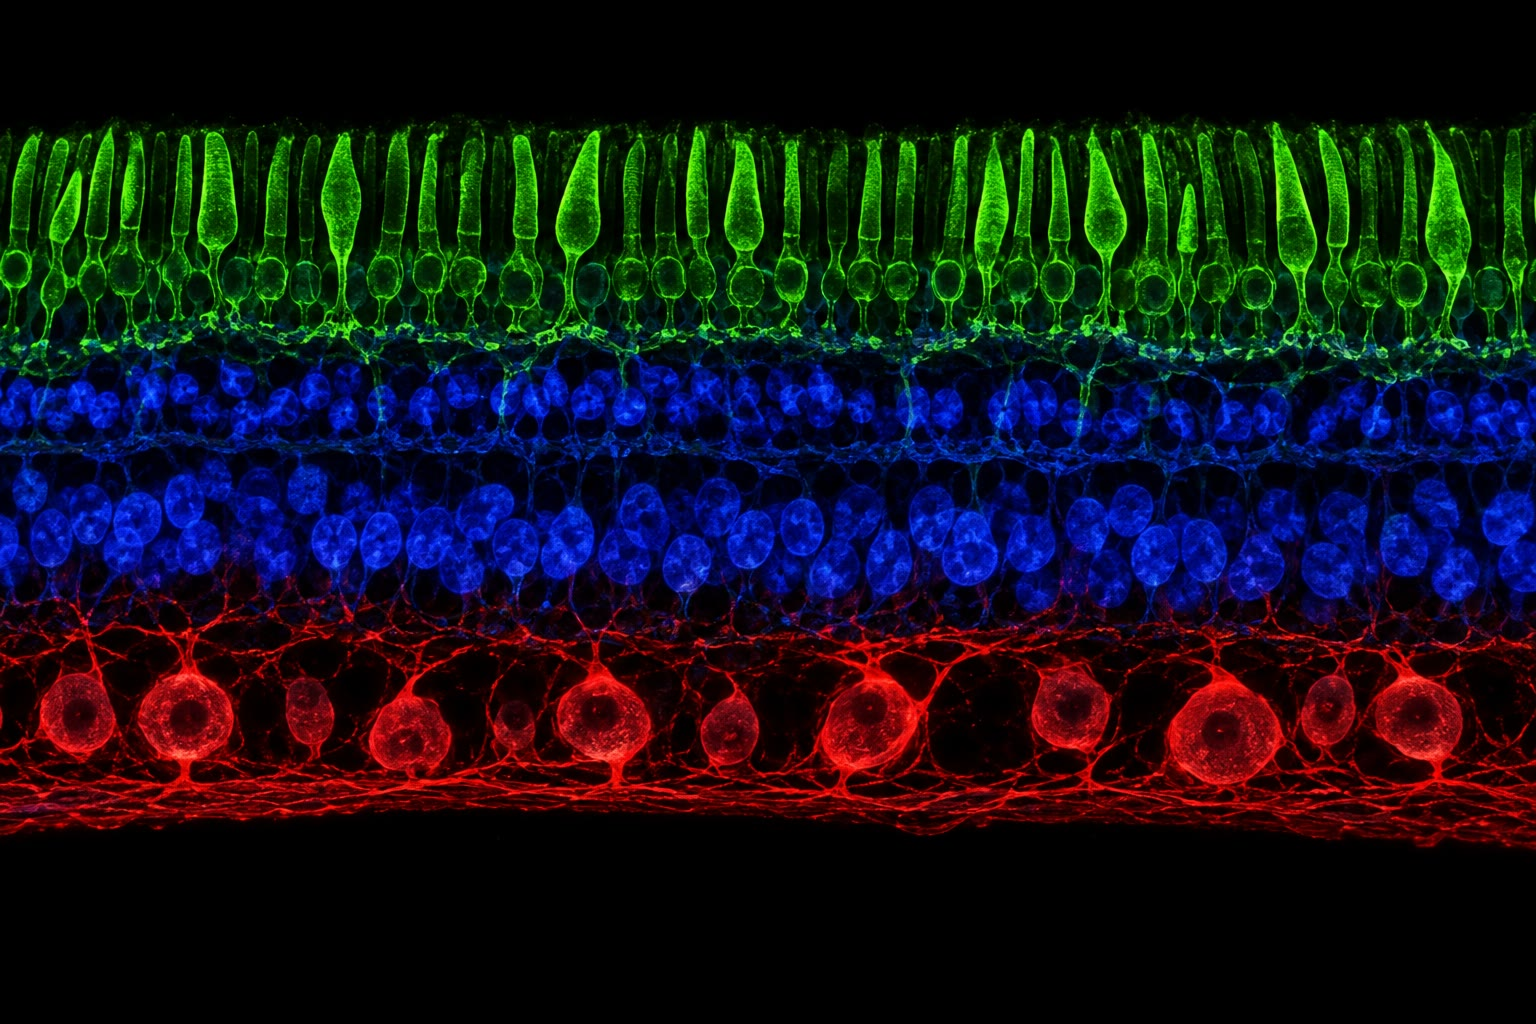
\includegraphics[width=0.46\linewidth]{images/book5/ai/b5-18-retina-section.jpg}\hspace{0.04\linewidth}
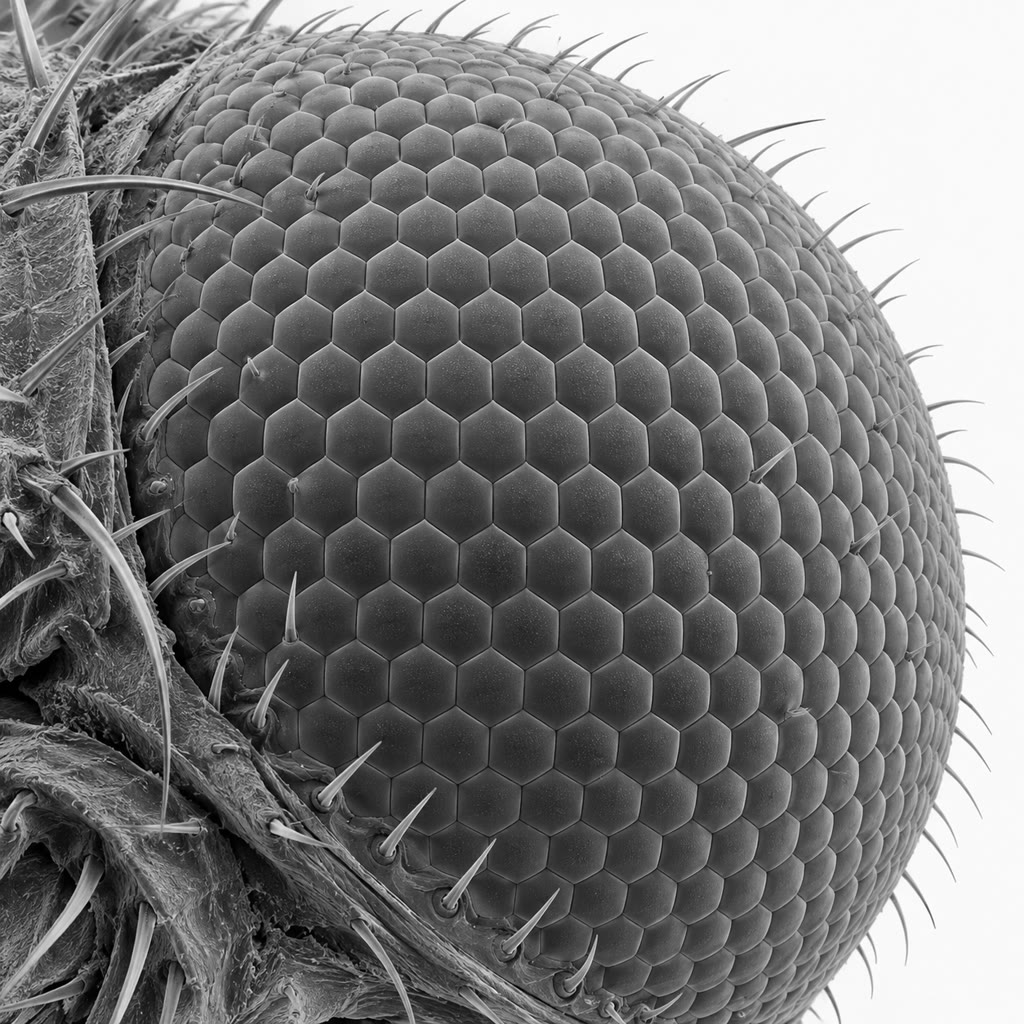
\includegraphics[width=0.36\linewidth]{images/book5/ai/b5-18-compound-eye.jpg}

{\small बाएँ: \omterm{def:b3:sensory-systems:retina}{दृष्टिपटल} की कोई काट, जिसमें पीछे की ओर प्रकाश-ग्राही
(हरे), फिर द्विध्रुवी तथा क्षैतिज कोशिकाएँ, फिर वे \omterm{def:b3:sensory-systems:retina}{गंडिका कोशिकाएँ}
(लाल) हैं जिनके तंत्रिकाक्ष मस्तिष्क के लिए निकलते हैं। दाएँ: किसी
मक्खी की संयुक्त आँख, सैकड़ों अलग-अलग लेंस, हर एक अपने ही ग्राहियों के
साथ --- उसी समस्या का कोई और हल।}
\end{omfigure}

\section{श्रवण और संतुलन}

\begin{definition}[कर्णावर्त]\label{def:b3:sensory-systems:cochlea}
\index{कर्णावर्त}\index{आधारकला}\index{स्वर-स्थानिकता}\index{रोम कोशिका}\index{स्थिरपक्ष्माभ}\index{शीर्ष-कड़ी}\index{डेसिबल}
ध्वनि कोई दाब-तरंग है; कान की समस्या हवा में कुछ ही दसियों
माइक्रोपास्कल के दाब-बदलाव पकड़ना और उन्हें बारंबारता से छाँटना है।
कर्णपटह और मध्य कान की तीन हड्डियाँ पटह के \qty{55}{mm^2} से आते बल को
अंडाकार गवाक्ष के \qty{3}{mm^2} पर सघन कर देती हैं, जिससे दाब कोई बीस
गुना बढ़ जाता है --- यही हवा और भीतरी कान के तरल के बीच का प्रतिबाधा-मेल
है, जिसके बिना अधिकांश ध्वनि परावर्तित हो जाती। \qty{35}{mm} लंबी उस
कुंडलित नली, यानी \emph{कर्णावर्त}, के भीतर वह दाब-तरंग \emph{आधारकला}
के अनुदिश चलती है, जो आधार पर सँकरी तथा कठोर और शीर्ष पर चौड़ी तथा ढीली
है; हर बारंबारता उस कला को किसी एक जगह सबसे अधिक कंपित करती है ---
ऊँची बारंबारताएँ आधार के पास, नीची शीर्ष के पास --- यानी कोई
\emph{स्वर-स्थानिक} मानचित्र, जिसे मस्तिष्क तारत्व की तरह पढ़ता है। उस
कला पर \emph{रोम कोशिकाएँ} बैठी हैं: किसी एक ही पंक्ति में \num{3500}
भीतरी रोम कोशिकाएँ, हर एक के सिर पर \emph{स्थिरपक्ष्माभों} का कोई
गट्ठर, जो महीन \emph{शीर्ष-कड़ियों} से सिरे-से-सिरे जुड़ा है; उस
गट्ठर को उसके सबसे ऊँचे \omterm{def:b3:cytoskeleton-motility:cilia}{पक्ष्माभ} की ओर झुकाने से वे कड़ियाँ खिंचती हैं
और माइक्रोसेकंडों के भीतर, बिना किसी द्वितीय संदेशवाहक के, धनायन
वाहिकाएँ खोल देती हैं, और पोटैशियम अंतःलसीका से भीतर बहता है, जिसके
असामान्य संघटन और $+\qty{80}{mV}$ विभव से \qty{150}{mV} का कोई चालक
बल मिलता है। भीतरी रोम कोशिकाएँ श्रवण तंत्रिका को संकेत देती हैं;
\num{12000} बाहरी रोम कोशिकाएँ, जो उसी गति से चलती हैं, प्रेरक प्रोटीन
प्रेस्टिन के ज़रिए ध्वनि के साथ सिकुड़ती और लंबी होती हैं तथा उस कला के
कंपन में ऊर्जा वापस पंप कर देती हैं --- यानी कोई ऐसा प्रवर्धक जो
सुरबंदी सौ गुना तीखी करता है और जो अधिकांश बहरेपन में विफल होता है।
तीव्रता \emph{डेसिबलों} में नापी जाती है: $L = 10\log_{10}
(I/I_{0})$, जिसमें $I_{0} = \qty{1e-12}{W/m^2}$ श्रवण की देहली है;
कान \qty{120}{dB} भर काम करता है, यानी तीव्रता में खरब गुना।
\end{definition}

\begin{omfigure}
\begin{tikzpicture}[every node/.style={font=\scriptsize}, >=stealth]
  % unrolled cochlea
  \begin{scope}
    \draw[thick, omDef, fill=omDef!10] (0,0.9) -- (7,1.4) -- (7,-1.4) -- (0,-0.9) -- cycle;
    \draw[very thick, omProp] (0,0.15) -- (7,-0.15); \draw[very thick, omProp] (0,-0.15) -- (7,0.15);
    \node[above] at (0.8,1.05) {आधार: सँकरा, कठोर}; \node[above] at (6.2,1.5) {शीर्ष: चौड़ा, ढीला};
    \node[left, align=right] at (-0.1,0) {अंडाकार गवाक्ष\\(रकाब से)};
    \foreach \x/\f in {0.9/\qty{16}{kHz}, 2.3/\qty{4}{kHz}, 3.8/\qty{1}{kHz}, 5.4/\qty{250}{Hz}, 6.6/\qty{60}{Hz}} { \draw[omThm, thick] (\x,-0.55) -- (\x,0.55); \node[below, omThm] at (\x,-0.65) {\f}; }
    \node[below, align=center] at (3.5,-1.7) {आधारकला (नारंगी): हर बारंबारता किसी\\एक जगह सबसे अधिक कंपती है --- स्वर-स्थानिकता};
  \end{scope}
  % hair cell mechanism
  \begin{scope}[xshift=8.2cm, yshift=-0.6cm]
    \draw[thick, fill=omMeth!20] (0,0) rectangle (1.6,1.2); \node[below] at (0.8,-0.05) {रोम कोशिका};
    \foreach \x/\h in {0.35/0.6, 0.65/0.85, 0.95/1.1, 1.25/1.35} \draw[very thick, omMeth!70!black] (\x,1.2) -- (\x,1.2+\h);
    \foreach \x/\h/\xx/\hh in {0.35/0.6/0.65/0.85, 0.65/0.85/0.95/1.1, 0.95/1.1/1.25/1.35} \draw[omThm, thick] (\x,1.2+\h) -- (\xx,1.2+\hh-0.1);
    \draw[->, thick] (1.9,2.3) -- (2.4,2.3) node[right, align=left, font=\tiny] {सबसे ऊँचे की ओर झुकाइए:\\शीर्ष-कड़ियाँ खिंचती हैं, वाहिकाएँ\\$\unit{\micro s}$ में खुलती हैं; K$^{+}$ घुसता है\\(\qty{150}{mV} चालक बल)};
    \node[above, align=center] at (0.8,2.7) {शीर्ष-कड़ियों (लाल) से\\जुड़े स्थिरपक्ष्माभ};
  \end{scope}
\end{tikzpicture}

{\small बाएँ: खोला गया \omterm{def:b3:sensory-systems:cochlea}{कर्णावर्त} --- \omterm{def:b3:sensory-systems:cochlea}{आधारकला} कठोर से ढीली की ओर
श्रेणीबद्ध है, और हर बारंबारता अपनी ही जगह पर शिखर छूती है। दाएँ: कोई
रोम-गट्ठर, जिसकी \omterm{def:b3:sensory-systems:cochlea}{शीर्ष-कड़ियाँ} गट्ठर के झुकने पर पारक्रमण-वाहिकाएँ
यांत्रिक रूप से खोल देती हैं।}
\end{omfigure}

\begin{proof}[प्रमाण-सामग्री]
फ़ोन बेकेशी (1940 का दशक) ने शवों के \omterm{def:b3:sensory-systems:cochlea}{कर्णावर्त} खोले, \omterm{def:b3:sensory-systems:cochlea}{आधारकला} पर
चाँदी के कण छिड़के और स्ट्रोबोस्कोपी प्रकाश में देखा कि शुद्ध स्वर कोई
ऐसी यात्री तरंग खड़ी करते हैं जिसका शिखर स्वर के जितना ऊँचा हो उतना ही
आधार के पास पड़ता है --- यानी स्थान-कूट, जिसके लिए उसे 1961 में नोबेल
पुरस्कार मिला। हडस्पेथ (1980 का दशक) ने किसी काँच-तंतु से कोई एक
रोम-गट्ठर धकेला और धारा अभिलिखित की: वह धक्के के \qty{10}{\micro s} के
भीतर बही, जो किसी भी एंज़ाइम-शृंखला के लिए कहीं अधिक तेज़ है, और इस
अनुपात में कि वह गट्ठर अपनी सबसे ऊँची पंक्ति की ओर कितना हिला, और वह
तब लोप हो गई जब \omterm{def:b3:sensory-systems:cochlea}{शीर्ष-कड़ियाँ} किसी कैल्सियम कीलेटक से काट दी गईं। द्वार
यांत्रिक है --- वह कड़ी उस वाहिका को खींचकर खोल देती है --- और इसीलिए
श्रवण सबसे तेज़ संवेदन है और इसीलिए उसका पारक्रमक उन तेज़ ध्वनियों से
नष्ट हो जाता है जो वे कड़ियाँ तोड़ देती हैं।
\end{proof}

\begin{example}[कान के आँकड़े]\label{ex:b3:sensory-systems:ear-numbers}
श्रवण की देहली पर \omterm{def:b3:sensory-systems:cochlea}{आधारकला} लगभग \qty{0.1}{nm} हिलती है और दाब का आयाम
\qty{20}{\micro Pa} है, यानी वायुमंडलीय का दो अरबवाँ भाग;
\qty{120}{dB} पर वह दाब दस लाख गुना अधिक है और उस कला की गति दसियों
नैनोमीटर। कोई जवान कान \qty{20}{Hz} से \qty{20}{kHz} तक सुनता है और
\qty{0.3}{\%} की दूरी पर पड़े स्वर अलग बता देता है, और स्थान-कूट का यह
विभेदन बाहरी \omterm{def:b3:sensory-systems:cochlea}{रोम कोशिकाएँ} तीखा करती हैं। श्रवण तंत्रिका के \num{30000}
तंतु लगभग \qty{4}{kHz} तक दाब-तरंग के साथ ताल में दगते हैं (कला-बंधन),
और दसियों माइक्रोसेकंडों की परिशुद्धि तक समय ढोते हैं, जिससे मस्तिष्क
किसी ध्वनि की दिशा दोनों कानों तक पहुँचने के अंतर से गणित लेता है ---
और वह अंतर \qty{10}{\micro s} जितना छोटा भी हो सकता है। संतुलन-अंग वही
\omterm{def:b3:sensory-systems:cochlea}{रोम कोशिकाएँ} काम में लेते हैं: \emph{अर्धवृत्ताकार नलिकाओं} में सिर
घूमने पर तरल का जड़त्व उन्हें झुका देता है (कोणीय त्वरण), और
कर्णाश्मरी अंगों में कैल्सियम कार्बोनेट के क्रिस्टलों की कोई परत उन्हें
गुरुत्व तथा रैखिक त्वरण से लाद देती है।
\end{example}

\begin{omfigure}
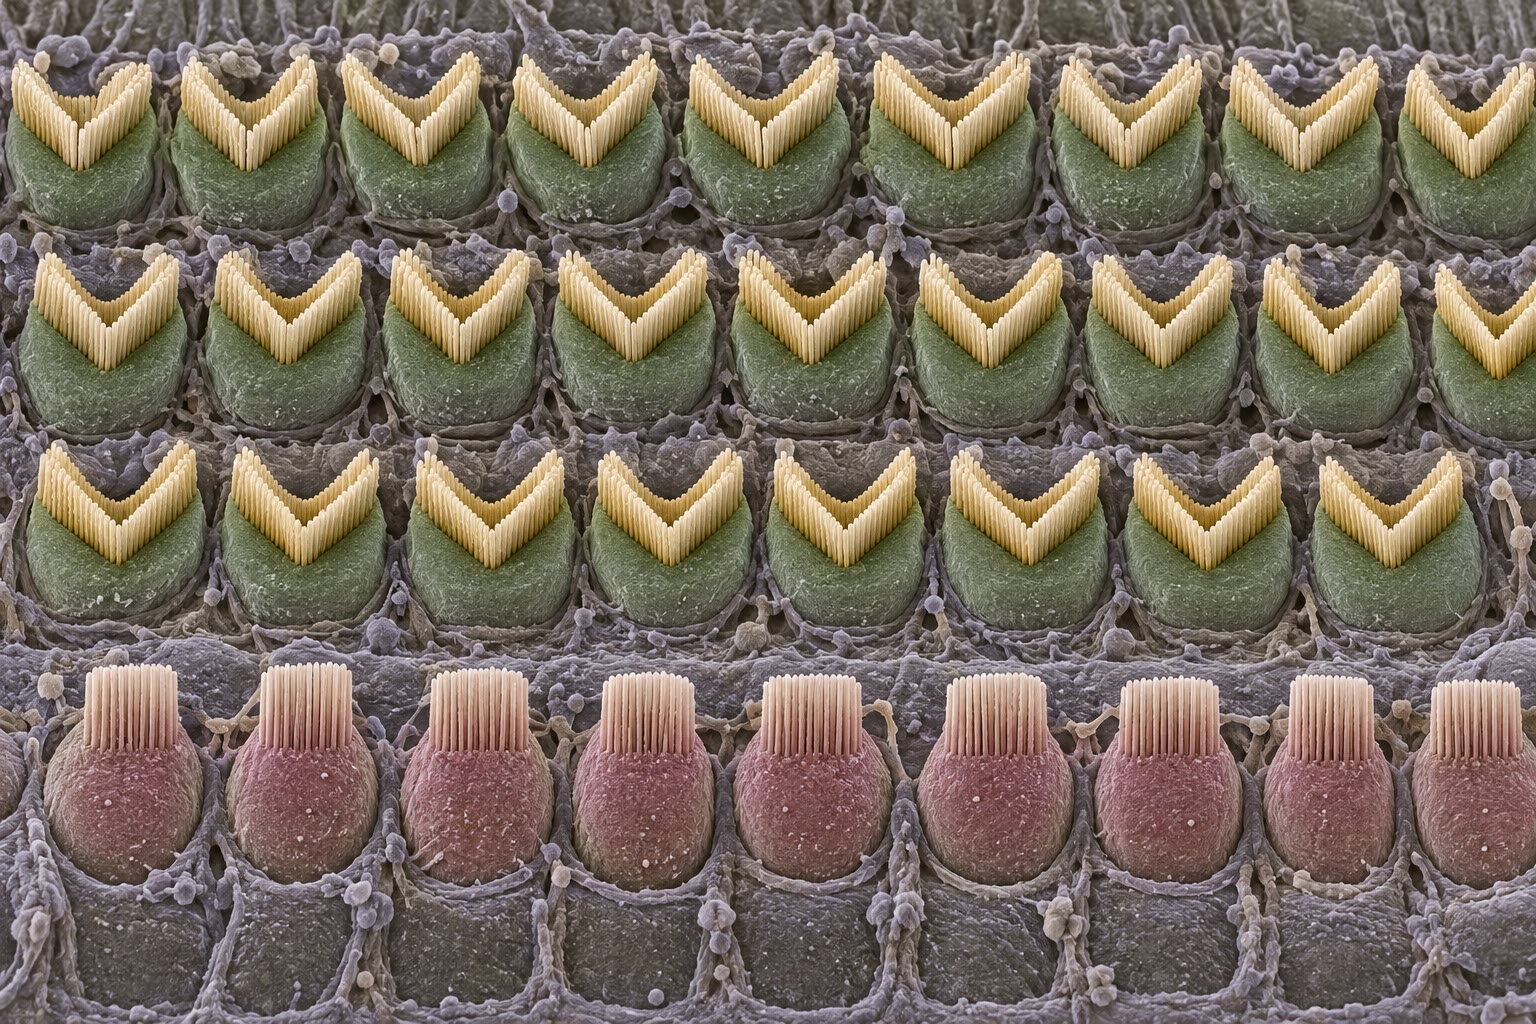
\includegraphics[width=0.54\linewidth]{images/book5/ai/b5-18-cochlea-hair-cells.jpg}

{\small कोर्टी का अंग ऊपर से: V-आकार के गट्ठरों वाली बाहरी \omterm{def:b3:sensory-systems:cochlea}{रोम
कोशिकाओं} की तीन पंक्तियाँ, भीतरी \omterm{def:b3:sensory-systems:cochlea}{रोम कोशिकाओं} की एक पंक्ति। हर गट्ठर
की \omterm{def:b3:sensory-systems:cochlea}{शीर्ष-कड़ियाँ} वाहिकाएँ खोलती हैं; बाहरी कोशिकाएँ प्रवर्धित करती हैं,
भीतरी बताती हैं।}
\end{omfigure}

\section{रासायनिक इंद्रियाँ}

\begin{definition}[घ्राण और स्वाद]\label{def:b3:sensory-systems:chemical}
\index{घ्राण ग्राही}\index{संचयात्मक कूट}\index{ग्लोमेरुलस}\index{स्वाद}
गंध नाक के ऊपरी हिस्से में उपकला के किसी टुकड़े से शुरू होती है, जहाँ
कोई एक करोड़ \emph{घ्राण संवेदी न्यूरॉन} मनुष्यों के लगभग $400$
(और किसी चूहे में \num{1100}, यानी दोनों में से किसी भी जीनोम का सबसे
बड़ा जीन-कुल) में से एक-एक \emph{घ्राण ग्राही} जीन अभिव्यक्त करते हैं
--- यानी G-प्रोटीन-युग्मित ग्राही, जो गंधद्रव्य अणुओं को किसी जेब में
बाँधते हैं और, चक्रीय AMP के ज़रिए, कोई वाहिका खोल देते हैं। हर ग्राही
कई गंधद्रव्य बाँधता है और हर गंधद्रव्य कई ग्राही, इसलिए कोई गंध कोई
\emph{संचयात्मक कूट} है, यानी उन $400$
ग्राही-प्रकारों भर में क्रियाशीलता का कोई प्रतिरूप, और किसी अणु में एक
कार्बन का बदलाव वह प्रतिरूप और वह गंध बदल देता है। किसी एक ग्राही को
अभिव्यक्त करते सारे न्यूरॉन अपने तंत्रिकाक्ष घ्राण बल्ब के उसी एक या
दो \emph{ग्लोमेरुलसों} तक भेजते हैं, इसलिए वह बल्ब कोई ऐसा मानचित्र
रखता है जिसमें हर गंध सक्रिय ग्लोमेरुलसों का कोई स्थानिक प्रतिरूप है,
जिसे प्रांतस्था बिना \omterm{def:b3:nervous-systems:plan}{चेतक} से गुज़रे पढ़ लेती है। स्वाद सरल है: पाँच
प्रकार, हर एक अपनी ही ग्राही कोशिकाओं से आता कोई \omterm{def:b3:sensory-systems:principles}{नामांकित तार} ---
मीठा, उमामी और कड़वा G-प्रोटीन-युग्मित ग्राहियों से (एक मीठा ग्राही,
एक उमामी, कोई पच्चीस कड़वे), नमकीन किसी सोडियम वाहिका से, खट्टा किसी
प्रोटॉन वाहिका से --- और जिसे हम स्वाद कहते हैं उसका बाकी सब गंध है,
जो मुँह के पिछले हिस्से से होकर नाक तक पहुँचती है।
\end{definition}

\begin{proof}[प्रमाण-सामग्री]
बक और ऐक्सल (1991) ने तर्क किया कि गंधद्रव्य-ग्राही ऐसे
G-प्रोटीन-युग्मित ग्राही होंगे जो केवल घ्राण उपकला में अभिव्यक्त होते
हों, और अपह्रासी प्राइमरों वाली PCR से उन्होंने ऐसे सैकड़ों जीनों का
कोई कुल पाया, जो वहीं अभिव्यक्त होते थे और कहीं नहीं --- यानी गंध के
ग्राही, जो सदी भर से अज्ञात थे। यथास्थान संकरण ने प्रति न्यूरॉन एक
ग्राही और एक जैसे न्यूरॉनों का एकल \omterm{def:b3:sensory-systems:chemical}{ग्लोमेरुलसों} पर अभिसरण दिखाया;
मालनिक, बक और सहयोगियों (1999) ने एकल न्यूरॉन अभिलिखित किए और दिखाया
कि हर गंधद्रव्य कई ग्राही-प्रकार सक्रिय करता था और हर ग्राही कई
गंधद्रव्य --- यानी वही \omterm{def:b3:sensory-systems:chemical}{संचयात्मक कूट}। बुशदिद और सहयोगियों (2014) ने
विषयों से मिश्रणों में भेद करवाया और आँका कि मनुष्य एक खरब से भी अधिक
गंधें अलग बता सकते हैं, जो आम धारणा के कुछ हज़ार से कहीं आगे है।
\end{proof}

\begin{proposition}[किसी संचयात्मक कूट की क्षमता]\label{prop:b3:sensory-systems:combinatorial}
\index{संचयात्मक कूट!क्षमता}
$R$ ग्राही-प्रकारों के साथ, जिनमें से हर एक या तो सक्रिय हो या चुप,
किसी गंध का प्रतिनिधित्व $2^{R}$ प्रतिरूपों में से किसी से भी हो सकता
है; $R = 400$ के साथ वह $10^{120}$ है, और यदि केवल ठीक $10$ सक्रिय
प्रकारों वाले प्रतिरूप गिने जाएँ तब भी $\binom{400}{10} \approx 3\times 10^{20}$
हैं। विभेदन को वह कूट नहीं, बल्कि ग्राहियों का शोर और मस्तिष्क का
पढ़ना सीमित करता है: प्रति गंध एक ग्राही वाला कोई नामांकित-तार कूट
$400$ गंधों की छूट देता, जबकि कोई \omterm{def:b3:sensory-systems:chemical}{संचयात्मक कूट} सूँघने को मौजूद अणुओं
से भी अधिक की। इसकी कीमत यह है कि कोई एक ग्राही अपने बूते मस्तिष्क को
बहुत कम बताता है; उस प्रतिरूप को पूरा-का-पूरा पढ़ना पड़ता है, और यही
ग्लोमेरुलसी मानचित्र तथा घ्राण प्रांतस्था करते हैं।
\end{proposition}

\begin{omfigure}
\begin{tikzpicture}[every node/.style={font=\scriptsize}, >=stealth]
  % receptor rows, odorant columns
  \foreach \i/\lab in {1/{ग्राही A}, 2/{ग्राही B}, 3/{ग्राही C}, 4/{ग्राही D}, 5/{ग्राही E}} \node[left] at (-0.1,-0.7*\i) {\lab};
  \foreach \j/\lab in {1/{हेक्सेनॉल}, 2/{हेप्टेनॉल}, 3/{ऑक्टेनॉल}, 4/{लिमोनीन}} \node[above, rotate=0] at (1.2*\j-0.6,-0.35) {\lab};
  \foreach \i/\j/\v in {1/1/100, 1/2/30, 2/1/60, 2/2/100, 2/3/50, 3/2/40, 3/3/100, 3/4/20, 4/3/70, 5/4/100, 1/4/30} \fill[omThm!\v] (1.2*\j-1.15,-0.7*\i-0.3) rectangle (1.2*\j-0.05,-0.7*\i+0.3);
  \foreach \i in {1,...,5} \foreach \j in {1,...,4} \draw[gray!50] (1.2*\j-1.15,-0.7*\i-0.3) rectangle (1.2*\j-0.05,-0.7*\i+0.3);
  \node[below, align=center] at (2.1,-4.1) {हर गंधद्रव्य ग्राहियों का कोई समुच्चय सक्रिय करता है,\\हर ग्राही गंधद्रव्यों का कोई समुच्चय:\\गंध वही स्तंभ है};
  % glomerular map
  \begin{scope}[xshift=9.2cm, yshift=-2.2cm]
    \draw[thick, omDef!60, fill=omDef!8] (0,0) ellipse (2.6 and 1.7); \node[above] at (0,1.75) {घ्राण बल्ब: ग्लोमेरुलस};
    \foreach \p in {(-1.8,0.6),(-1.0,1.0),(-0.2,0.7),(0.8,1.0),(1.7,0.5),(-1.6,-0.4),(-0.6,-0.6),(0.4,-0.3),(1.3,-0.7),(0.1,0.2)} \draw[omDef!70, fill=omDef!25] \p circle (0.25);
    \fill[omThm!80] (-1.0,1.0) circle (0.25); \fill[omThm!50] (0.4,-0.3) circle (0.25); \fill[omThm!80] (1.7,0.5) circle (0.25);
    \node[below, align=center] at (0,-1.8) {किसी एक ग्राही-प्रकार के सारे न्यूरॉन\\एक ही ग्लोमेरुलस पर मिलते हैं: गंध कोई\\स्थानिक प्रतिरूप (लाल) है, जिसे प्रांतस्था पढ़ती है};
  \end{scope}
\end{tikzpicture}

{\small गंध का \omterm{def:b3:sensory-systems:chemical}{संचयात्मक कूट}। बाएँ: कोई ग्राही-बनाम-गंधद्रव्य आव्यूह,
जिसमें हर गंध किसी स्तंभ में उतरता कोई प्रतिरूप है। दाएँ: वही प्रतिरूप
बल्ब के \omterm{def:b3:sensory-systems:chemical}{ग्लोमेरुलसों} पर बिछा हुआ।}
\end{omfigure}

\begin{omfigure}
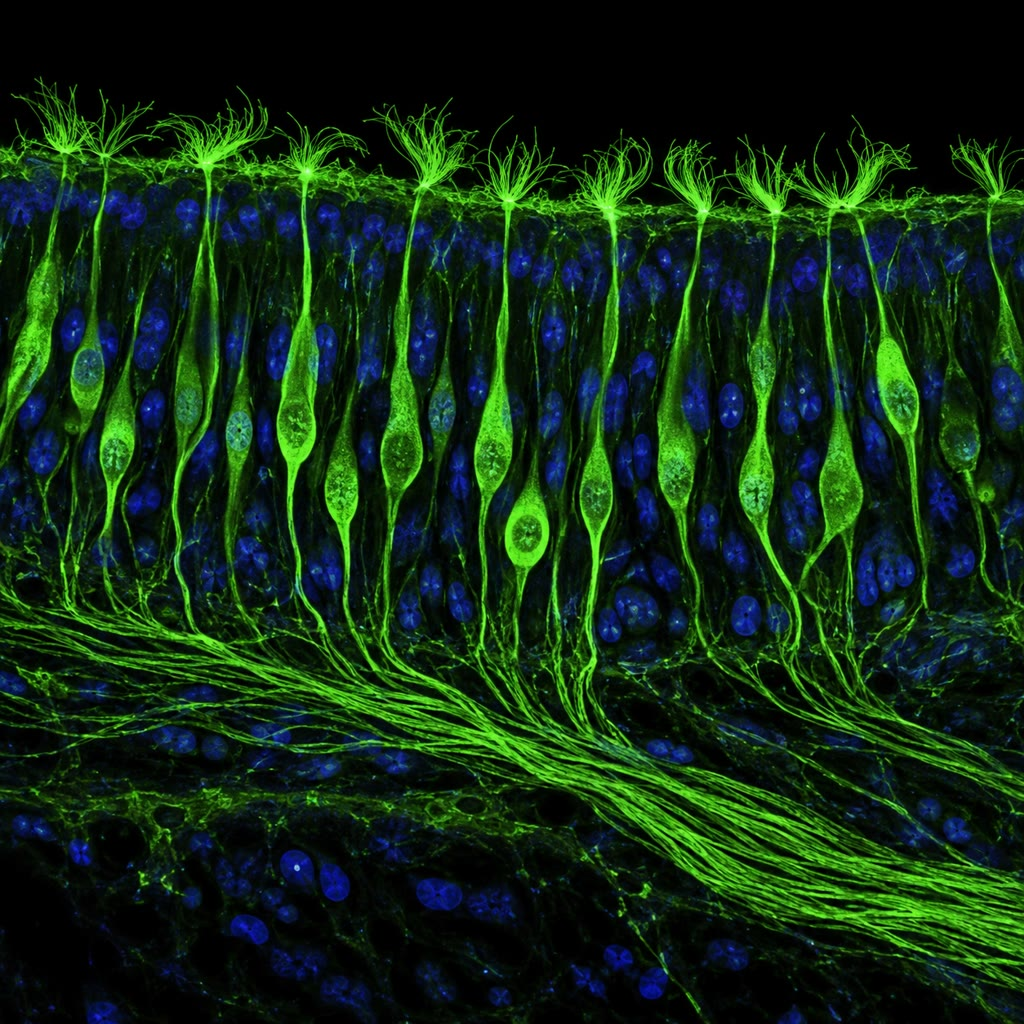
\includegraphics[width=0.40\linewidth]{images/book5/ai/b5-18-olfactory-epithelium.jpg}

{\small घ्राण उपकला: संवेदी न्यूरॉन (हरे), जिनकी पक्ष्माभी द्रुमिकाएँ
पृष्ठ पर हैं, जहाँ गंधद्रव्य बँधते हैं, और जिनके तंत्रिकाक्ष नीचे बल्ब
की ओर गट्ठर बनाते हैं। हर न्यूरॉन उन चार सौ में से एक ग्राही जीन
अभिव्यक्त करता है।}
\end{omfigure}

\section{स्पर्श, तापमान, पीड़ा और वे इंद्रियाँ जो हममें नहीं}

\begin{definition}[कायसंवेदन]\label{def:b3:sensory-systems:somato}
\index{यांत्रिक ग्राही}\index{पीज़ो वाहिका}\index{TRP वाहिका}\index{पीड़ाग्राही}\index{स्वांगस्थिति बोध}
त्वचा में कई तरह के \emph{यांत्रिक ग्राही} हैं, हर एक अपने ही संपुट
में समाप्त होता कोई तंत्रिकाक्ष: महीन दाब और गठन के लिए मर्केल
कोशिकाएँ (धीरे अनुकूलित होतीं, छोटे क्षेत्र), हलके स्पर्श तथा फिसलन के
लिए माइसनर कणिकाएँ (तेज़ी से अनुकूलित होतीं), कंपन के लिए त्वचा में
गहरी पैसिनी कणिकाएँ (बहुत तेज़ी से अनुकूलित होतीं, विशाल क्षेत्र), और
तनाव के लिए रफ़िनी सिरे। उनमें से अधिकांश का पारक्रमक \emph{पीज़ो2}
है, यानी कोई विशाल आयन-वाहिका, जिसके पंखों का कोई चक्र है और जो झिल्ली
के खिंचने पर खुल जाती है; उसके बिना स्पर्श और देह-स्थिति का बोध चला
जाता है, और वही वाहिका फुफ्फुसों तथा मूत्राशय में उनका भरना भाँपती है।
\emph{तापमान} TRP कुल की उन वाहिकाओं से भाँपा जाता है जो भिन्न परासों
पर सुरबद्ध हैं --- TRPV1, जो \qty{43}{\celsius} से ऊपर की ऊष्मा से और
कैप्सेसिन से खुलती है, और इसीलिए मिर्च ``तीखी'' लगती है; TRPM8, जो ठंड
से और मेंथॉल से खुलती है --- और \emph{पीड़ा} मुक्त तंत्रिका-सिरों से,
यानी \emph{पीड़ाग्राहियों} से, जो हानिकारक ऊष्मा, दाब या रसायनों
(प्रोटॉन, ATP, ब्रैडीकाइनिन) पर अनुक्रिया देते हैं और जिनकी देहलियाँ
\omterm{def:b3:innate-immunity:inflammation}{शोथ} से नीची हो जाती हैं (\cref{ch:b3:innate-immunity})।
\emph{स्वांगस्थिति बोध}, यानी यह बोध कि अंग कहाँ हैं,
\cref{ch:b3:nervous-systems} के पेशी-तर्कुओं तथा कंडरा-अंगों से और
जोड़-संपुटों के पीज़ो2 से आता है। ग्राहियों का घनत्व तीक्ष्णता तय करता
है: \qty{2}{mm} की दूरी पर पड़े दो बिंदु उँगली के सिरे पर अलग बताए जाते
हैं, और पीठ पर \qty{40}{mm} की दूरी पर।
\end{definition}

\begin{method}[किसी संवेदन का मापन]\label{met:b3:sensory-systems:psychophysics}
\index{मनोभौतिकी}\index{देहली}\index{द्विबिंदु विभेदन}
किसी संवेदी चैनल का लक्षण-वर्णन करने के लिए: (1) श्रेणीबद्ध तीव्रता के
उद्दीपक अनेक बार प्रस्तुत करके और पकड़े गए अंश को फिट करके
\emph{निरपेक्ष देहली} खोजिए --- यानी वह तीव्रता जो आधी बार पकड़ी जाए
--- जैसा हेख़्ट ने किया; (2) कई तीव्रताओं पर \emph{अंतर-देहली} खोजिए और
\omterm{thm:b3:sensory-systems:weber}{वेबर का नियम} जाँचिए; (3) बदलती दूरी पर दो उद्दीपकों से \emph{स्थानिक
तीक्ष्णता} मानचित्रित कीजिए (त्वचा पर द्विबिंदु परीक्षण, \omterm{def:b3:sensory-systems:retina}{दृष्टिपटल} पर
कोई जालिका); (4) टिमटिमाहट या चटकों से \emph{कालिक तीक्ष्णता}
मानचित्रित कीजिए (दिन की दृष्टि में टिमटिमाहट लगभग \qty{60}{Hz} पर
जुड़ जाती है); (5) किसी प्राणी में, वही उद्दीपक लगाते हुए एकल अभिवाही
तंतुओं से अभिलेख लीजिए और तंत्रिकीय देहलियाँ व्यवहारिक देहलियों से
मिलाइए --- मनोभौतिकी और शरीरक्रिया को सहमत होना चाहिए, और जहाँ वे न
हों वहाँ का अंतर वही है जो मस्तिष्क जोड़ता है।
\end{method}

\begin{remark}[दूसरे प्राणी, दूसरी इंद्रियाँ]\label{rem:b3:sensory-systems:others}
यहाँ का हर संवेदन किसी न किसी प्राणी में और आगे तक ले जाया गया है, और
कुछ इंद्रियाँ ऐसी भी हैं जो हममें नहीं। शार्क और शंकुश किसी शिकार की
धड़कन के माइक्रोवोल्ट क्षेत्र जेली भरी नलिकाओं से भाँपते हैं; विद्युत्
मछलियाँ अपने ही क्षेत्र के विरूपण पढ़कर अँधेरे में देखती हैं।
गड्ढेदार सर्प अवरक्त-संवेदी गड्ढों से गरम शिकार का प्रतिबिंब बनाते
हैं; चमगादड़ और डॉल्फ़िन प्रतिध्वनि-स्थानन करते हैं, अपनी ही पुकारों
की गूँजों को कुछ माइक्रोसेकंडों तक समयबद्ध करते हैं और किसी पतंगे का
पीछा करने के लिए पुकार की बारंबारता साधते हैं; मधुमक्खियाँ पराबैंगनी
और आकाश-प्रकाश का ध्रुवण देखती हैं और उसी से दिशा पाती हैं; प्रवासी
पक्षी और कछुए पृथ्वी का चुंबकीय क्षेत्र किसी ऐसे तंत्र से भाँपते हैं
जिस पर अब भी बहस है। किसी कुत्ते की नाक में हमसे चालीस गुना ग्राही
न्यूरॉन हैं और उन्हें पढ़ने के लिए उसके मस्तिष्क का तिहाई; कोई उल्लू
बर्फ़ के नीचे दबे चूहे को सुन लेता है। सिद्धांत नहीं बदलते --- कोई
पारक्रमक, कोई \omterm{def:b3:sensory-systems:principles}{नामांकित तार}, कोई कूट, निचोड़, कोई मानचित्र --- और यह
विविधता वही है जो विकास ने उनसे किया है।
\end{remark}

\section{अभ्यास}

\begin{exercise}[$\star$]\label{exo:b3:sensory-systems:1}
समझाइए कि मस्तिष्क कैसे जानता है कि आवेगों की कोई रेल आँख से आई है या
कान से, जबकि वे आवेग एक जैसे हैं।
\end{exercise}

\begin{exercise}[$\star$]\label{exo:b3:sensory-systems:2}
प्रकाश किसी प्रकाश-ग्राही को अतिध्रुवित क्यों करता है, और अँधेरे की
धारा क्या है?
\end{exercise}

\begin{exercise}[$\star$]\label{exo:b3:sensory-systems:3}
कोई फुसफुसाहट \qty{20}{dB} की है, कोई बातचीत \qty{60}{dB} की, कोई रॉक
संगीत-सभा \qty{110}{dB} की। हर एक की तीव्रता W/m$^{2}$ में निकालिए और
सबसे तेज़ तथा सबसे धीमी का अनुपात।
\end{exercise}

\begin{exercise}[$\star$]\label{exo:b3:sensory-systems:4}
\omterm{def:b3:sensory-systems:chemical}{स्वाद} के पाँचों प्रकार और उनके ग्राही-प्रकार बताइए, और समझाइए कि कोई
ज़ुकाम भोजन का ``\omterm{def:b3:sensory-systems:chemical}{स्वाद}'' क्यों रोक देता है।
\end{exercise}

\begin{exercise}[$\star\star$]\label{exo:b3:sensory-systems:5}
भार के लिए वेबर का अंश $0.02$ है। \qty{100}{g} के किसी भार से शुरू
करके, उसके और \qty{10}{kg} के बीच कितने बस-ध्यानयोग्य पग पड़ते हैं?
फ़ेख़नर का सूत्र काम में लीजिए और गुणक $1.02$ के पग गिनकर जाँचिए।
\end{exercise}

\begin{exercise}[$\star\star$]\label{exo:b3:sensory-systems:6}
\cref{thm:b3:sensory-systems:hecht} का उपयोग करते हुए $P_{\text{दिखना}}$
निकालिए, $a = 2$, $6$ और $12$ अवशोषित फ़ोटॉनों के लिए, जब देहली
$n = 6$ हो। किस $a$ पर वह कौंध आधी बार दिखती है? यदि कॉर्निया पर आते
फ़ोटॉनों का \qty{10}{\%} अवशोषित हो, तो उस कौंध को कितने पहुँचाने पड़ेंगे?
\end{exercise}

\begin{exercise}[$\star\star$]\label{exo:b3:sensory-systems:7}
मध्य कान \qty{55}{mm^2} से आते बल को $1.3$ के किसी उत्तोलक के साथ
\qty{3}{mm^2} पर सघन करता है। दाब कितने गुना बढ़ता है, और \omterm{def:b3:sensory-systems:cochlea}{डेसिबलों} में
कितना? जिस व्यक्ति की मध्य-कान की हड्डियाँ जुड़ गई हों (कर्णकाठिन्य)
उसका कान दसियों \omterm{def:b3:sensory-systems:cochlea}{डेसिबल} मंद क्यों होता है?
\end{exercise}

\begin{exercise}[$\star\star$]\label{exo:b3:sensory-systems:8}
समझाइए कि किसी \omterm{def:b3:sensory-systems:cochlea}{रोम कोशिका} की पारक्रमण-धारा माइक्रोसेकंडों में क्यों
प्रकट होती है जबकि किसी प्रकाश-ग्राही की दसियों मिलीसेकंड लेती है, और
हर संवेदन को अपने अभिकल्प से क्या मिलता है।
\end{exercise}

\begin{exercise}[$\star\star$]\label{exo:b3:sensory-systems:9}
किसी चूहे के \num{1100} ग्राही-प्रकार हैं और किसी मनुष्य के $400$। यदि
कोई गंध उन प्रकारों का लगभग \qty{5}{\%} सक्रिय करे, तो ठीक उतने ही
आकार के कितने प्रतिरूप हर एक के पास उपलब्ध हैं ($\binom{R}{k}$ काम में
लीजिए, जिसमें $k = 0.05R$ हो, और स्टर्लिंग का सन्निकटन
$\ln\binom{R}{k} \approx R\,H(k/R)$, जिसमें
$H(p) = -p\ln p - (1-p)\ln(1-p)$)?
\end{exercise}

\begin{exercise}[$\star\star\star$]\label{exo:b3:sensory-systems:10}
कोई \omterm{def:b3:sensory-systems:retina}{शलाका} अँधेरे में हर \qty{40}{s} में एक बार स्वतःस्फूर्त ढंग से
कोई \omterm{def:b3:sensory-systems:retina}{रोडॉप्सिन} समावयवित कर देती है। $500$ \omterm{def:b3:sensory-systems:retina}{शलाकाओं} के किसी टुकड़े को
\qty{0.1}{s} की खिड़की भर देखने पर स्वतःस्फूर्त घटनाओं की माध्य संख्या
क्या है, और यह प्रायिकता कि संयोग से छह या अधिक घटें? समझाइए कि
मस्तिष्क देहली लगभग छह पर क्यों रखता है, एक पर नहीं।
\end{exercise}

\begin{exercise}[$\star\star\star$]\label{exo:b3:sensory-systems:11}
श्रवण तंत्रिका अपने आवेग \qty{4}{kHz} तक ध्वनि की कला से बाँधती है,
जिसमें लगभग \qty{20}{\micro s} का कंपन रहता है। ध्वनि \qty{340}{m/s}
पर चलती है और कान \qty{20}{cm} की दूरी पर हैं। सबसे बड़ा अंतःकर्णी
विलंब क्या है, \qty{10}{\micro s} का विभेदन मध्य-रेखा के पास कौन-सा
कोणीय विभेदन देता है, और \qty{4}{kHz} से ऊपर समय नहीं बल्कि स्थान-कूट
क्यों काम आता है?
\end{exercise}

\begin{exercise}[$\star\star\star$]\label{exo:b3:sensory-systems:12}
\omterm{def:b3:sensory-systems:principles}{पार्श्व निरोध} किसी एक-सी धूसर सतह को, जो किसी गहरी सतह के बगल में हो,
सीमा पर हलका दिखा देता है। ग्राहियों की कोई ऐसी पंक्ति प्रतिरूपित
कीजिए जिसमें हर एक अपने ही प्रकाश $I_{i}$ से उत्तेजित हो और हर पड़ोसी
के प्रकाश के किसी अंश $w$ से निरोधित,
$r_{i} = I_{i} - w(I_{i-1} + I_{i+1})$, और $I = 1$ से $I = 2$ के किसी
पग के आर-पार अनुक्रिया निकालिए, $w = 0.2$ के साथ। इससे \omterm{def:b3:sensory-systems:retina}{दृष्टिपटल} को क्या
मिलता है और क्या खोता है?
\end{exercise}

\section{समस्या: दूर से दिखती एक मोमबत्ती}

\begin{problem}[{सप्तांत समस्या --- किसी दूर की आँख में गिने गए
मोमबत्ती के फ़ोटॉन, प्वासों सांख्यिकी और शलाका के प्रवर्धक से निकाला
गया कौंध का संसूचन, किसी संगीत-सभा के डेसिबल कर्णपटह की गति और रोम
कोशिका की धारा में बदले हुए, और किसी नाक का कूट गिना हुआ, जिसका अंत उस
दूरी पर होता है जहाँ तक वह मोमबत्ती दिखती है, कर्णपटह पर पड़ते दाब पर,
और उन प्रतिरूपों पर जो कोई नाक बना सकती है}]
\label{pb:b3:sensory-systems:1}
आँकड़े: कोई मोमबत्ती \qty{550}{nm} पर दृश्य प्रकाश के लगभग
\qty{0.01}{W} छोड़ती है (फ़ोटॉन की ऊर्जा $3.6\times 10^{-19}$ J)।
अँधेरे की अभ्यस्त कोई पुतली \qty{7}{mm} चौड़ी है; आँख में घुसते
फ़ोटॉनों का \qty{10}{\%} \omterm{def:b3:sensory-systems:retina}{रोडॉप्सिन} से अवशोषित होता है; आँख
\qty{0.1}{s} पर समाकलन करती है; देहली $6$ अवशोषित फ़ोटॉन है। हर
अवशोषित फ़ोटॉन $200$ वाहिकाएँ बंद कर देता है और अँधेरे की धारा
\qty{0.2}{s} के लिए \qty{1}{pA} घटा देता है; किसी \omterm{def:b3:sensory-systems:retina}{शलाका} की अँधेरे की
धारा \qty{30}{pA} है। ध्वनि: $I_{0} =
\qty{1e-12}{W/m^2}$; कर्णपटह का क्षेत्रफल \qty{55}{mm^2}; देहली पर
\qty{5}{\micro m} ऊँचाई का कोई रोम-गट्ठर \qty{0.3}{nm} विक्षेपित होता
है। घ्राण: $R = 400$ ग्राही; किसी \omterm{def:b3:sensory-systems:cochlea}{रोम कोशिका} की पारक्रमण-धारा संतृप्ति
पर \qty{100}{pA} है।

\medskip
\noindent\textbf{भाग I --- फ़ोटॉन।}
\begin{enumerate}
  \item वह मोमबत्ती प्रति सेकंड कितने फ़ोटॉन छोड़ती है?
  \item दूरी $d$ पर वे फ़ोटॉन $4\pi d^{2}$ क्षेत्रफल के किसी गोले पर
        फैल जाते हैं। \qty{1}{km} पर प्रति सेकंड कितने पुतली में घुसते
        हैं? \qty{10}{km} पर?
  \item हर दूरी पर एक समाकलन-खिड़की में कितने अवशोषित होते हैं? क्या वह
        मोमबत्ती दिखती है (देहली $6$)?
  \item वह दूरी खोजिए जिस पर किसी खिड़की में माध्य अवशोषित संख्या
        $6$ के बराबर हो। प्वासों सांख्यिकी के साथ, वहाँ खिड़कियों का
        कितना अंश देहली पार करता है?
  \item प्रश्न 4 की दूरी पर, यह प्रायिकता क्या है कि किसी दी
        \qty{0.1}{s} खिड़की में एक भी फ़ोटॉन न हो? कोई मंद तारा
        टिमटिमाता क्यों लगता है?
  \item पूरे चाँद में वही \omterm{def:b3:sensory-systems:retina}{शलाकाएँ} आकाश से प्रति खिड़की $10^{4}$ फ़ोटॉन
        अवशोषित करती हैं। समझाइए कि तब \qty{10}{km} की वह मोमबत्ती
        क्यों नहीं दिखती, जबकि वह उतने ही फ़ोटॉन पहुँचाती है।
\end{enumerate}

\medskip
\noindent\textbf{भाग II --- \omterm{def:b3:sensory-systems:retina}{शलाका} का प्रवर्धक।}
\begin{enumerate}[resume]
  \item एक फ़ोटॉन $200$ वाहिकाएँ बंद करता है और धारा \qty{1}{pA} घटा
        देता है। कोई एक वाहिका कितनी धारा ढोती है, और वह प्रति सेकंड
        कितने धनायन हुए ($e = \qty{1.6e-19}{C}$)?
  \item एक फ़ोटॉन अँधेरे की धारा का कितना अंश हटा देता है? कितने एक साथ
        आते फ़ोटॉन उस \omterm{def:b3:sensory-systems:retina}{शलाका} को पूरी तरह बंद कर देंगे (संतृप्ति)?
  \item वह अनुक्रिया \qty{0.2}{s} चलती है। एक फ़ोटॉन कितने धनायनों को
        भीतर आने से रोक देता है? प्रति फ़ोटॉन आवेश में लाभ क्या है?
  \item दिन के उजाले में किसी \omterm{def:b3:sensory-systems:retina}{शलाका} तक प्रति सेकंड $10^{5}$ फ़ोटॉन
        पहुँचते हैं। उसका क्या होता है, और \omterm{def:b3:sensory-systems:retina}{शंकु}, जो कम अनुकूलित और कम
        संतृप्त होते हैं, दिन के उजाले के ग्राही क्यों हैं?
  \item \omterm{def:b3:sensory-systems:retina}{शंकुओं} को संकेत देने के लिए लगभग $100$ फ़ोटॉन चाहिए।
        संवेदनशीलता और गति के बीच के सौदे के हिसाब से समझाइए कि \omterm{def:b3:sensory-systems:retina}{शंकु}
        \qty{20}{ms} में और \omterm{def:b3:sensory-systems:retina}{शलाकाएँ} \qty{200}{ms} में क्यों अनुक्रिया
        देती हैं।
  \item कोई \omterm{def:b3:sensory-systems:retina}{रोडॉप्सिन} \qty{40}{s} में एक बार स्वतःस्फूर्त ढंग से
        समावयवित होता है। किसी आँख की $10^{8}$ \omterm{def:b3:sensory-systems:retina}{शलाकाओं} भर में
        \omterm{def:b3:sensory-systems:retina}{दृष्टिपटल} प्रति सेकंड कितने झूठे फ़ोटॉन बनाता है, और उससे
        अँधेरे में बैठी आँख शोर से अंधी क्यों नहीं हो जाती? (देहली और
        \omterm{def:b3:sensory-systems:principles}{ग्राही क्षेत्र} का ध्यान कीजिए।)
\end{enumerate}

\medskip
\noindent\textbf{भाग III --- \omterm{def:b3:sensory-systems:cochlea}{डेसिबल}।}
\begin{enumerate}[resume]
  \item \qty{110}{dB} की कोई संगीत-सभा: W/m$^{2}$ में तीव्रता और किसी
        एक कर्णपटह पर पड़ती शक्ति।
  \item दो घंटे की किसी संगीत-सभा में कर्णपटह कितनी ध्वनिक ऊर्जा पाता
        है? किसी गिरती वर्षा-बूँद की ऊर्जा (\qty{1e-4}{J}) से तुलना
        कीजिए।
  \item \qty{0}{dB} पर श्रवण की देहली: कर्णपटह पर शक्ति और प्रति
        \qty{10}{ms} ऊर्जा --- किसी एक दृश्य फ़ोटॉन की ऊर्जा से तुलना
        कीजिए।
  \item वह रोम-गट्ठर \qty{5}{\micro m} की ऊँचाई पर देहली पर
        \qty{0.3}{nm} विक्षेपित होता है। वह कितने अंश का कोण हुआ? उस
        विक्षेप की तुलना किसी हाइड्रोजन परमाणु के व्यास
        (\qty{0.1}{nm}) से कीजिए।
  \item \qty{85}{dB} से ऊपर लंबा संसर्ग \omterm{def:b3:sensory-systems:cochlea}{रोम कोशिकाएँ} क्षतिग्रस्त कर
        देता है, और स्तनियों में \omterm{def:b3:sensory-systems:cochlea}{रोम कोशिकाएँ} फिर नहीं बनतीं।
        \qty{110}{dB} पर दो घंटे \qty{85}{dB} पर कितने घंटों जितनी
        ऊर्जा पहुँचाते हैं?
  \item श्रवण की परास \qty{120}{dB} है। यदि तीव्रता के लिए वेबर का अंश
        लगभग $0.25$ (यानी एक \omterm{def:b3:sensory-systems:cochlea}{डेसिबल}) हो, तो वह प्रबलता के कितने
        बस-ध्यानयोग्य पग हुए?
\end{enumerate}

\medskip
\noindent\textbf{भाग IV --- गंध का कूट।}
\begin{enumerate}[resume]
  \item $400$ ग्राहियों के साथ, जिनमें हर एक चालू या बंद हो, कितने
        प्रतिरूप? उत्तर दस की किसी घात के रूप में लिखिए।
  \item यदि कोई गंध प्रायः $20$ ग्राही सक्रिय करती हो, तो ऐसे कितने
        भिन्न प्रतिरूप हैं ($\binom{400}{20}$, स्टर्लिंग या लघुगणक काम
        में लीजिए)?
  \item दो गंधद्रव्य $15$ ग्राही साझा करते हैं, अपने $20$ में से। कूट
        में उनकी दूरी का कोई माप सुझाइए और समझाइए कि वे एक जैसी गंध
        क्यों देते हैं।
  \item मनुष्य लगभग एक खरब गंधें अलग पहचानते हैं। वह प्रश्न 20 के
        प्रतिरूपों का कितना अंश है, और उस संख्या को कूट की क्षमता से
        इतना नीचे क्या सीमित करता है?
  \item \num{1100} ग्राहियों वाला कोई चूहा: $20$ के प्रतिरूप किसी
        मनुष्य से कितने गुना अधिक, दस की किसी घात के रूप में?
  \item कोई उत्परिवर्तन एक ग्राही जीन विलोपित कर देता है। सूँघने की
        सामान्य क्षमता पर और उस एक गंधद्रव्य के प्रत्यक्षण पर, जो उस
        ग्राही से ज़ोर से बँधता है, उसका असर बताइए (विशिष्ट अगंधता)।
  \item सारांश दीजिए: वह दूरी जिस पर वह मोमबत्ती दिखती है (प्रश्न~4),
        देहली पर \qty{10}{ms} में कर्णपटह तक पहुँचती ध्वनिक ऊर्जा
        (प्रश्न~15), और बीस-ग्राही प्रतिरूपों की वह संख्या जो कोई मानव
        नाक बना सकती है (प्रश्न~20)।
\end{enumerate}
\end{problem}
